\documentclass[11pt,a4paper]{article}

\usepackage[a4paper,margin=1in]{geometry}
\usepackage{amsmath}
\usepackage{booktabs}
\usepackage{longtable}
\usepackage{graphicx}
\usepackage{float}
\usepackage{hyperref}
\usepackage{caption}
\usepackage{subcaption}
\usepackage{array}
\usepackage{setspace}

\hypersetup{
  colorlinks=true,
  linkcolor=blue,
  urlcolor=blue,
  citecolor=blue
}

\setstretch{1.12}

\title{Portugal's Public-Debt Interest Burden: Measurement, Dynamics, and Comparative Evidence}
\author{Diogo Ribeiro}
\date{July 2026}

\begin{document}
\maketitle

\begin{abstract}
This report presents a reproducible empirical assessment of Portugal's
general-government interest burden. The object of study is interest payable by
the general-government sector, measured in euros and as a percentage of nominal
GDP. The main harmonised series is built from Eurostat ESA 2010 national
accounts from 1995 onward; an AMECO linked extension is retained for pre-1995
historical context, with explicit accounting-basis labels. The analysis
documents the long decline in the interest burden from the mid-1990s, the
temporary reversal during the sovereign-debt crisis, the post-2015 compression
of the effective interest rate, and the recent tension between higher market
rates and a declining debt ratio. In 2025 Portugal paid EUR 5.96 billion in
general-government interest, equal to 1.90 percent of GDP, while gross debt was
89.70 percent of GDP and the implicit interest rate was 2.18 percent. In the
latest comparator panel Portugal ranked fourth of seven non-aggregate countries
by interest expenditure as a percentage of GDP. The report combines descriptive
statistics, accounting identities, debt-dynamics decomposition, cross-country
comparison, and deterministic rate-shock simulations.
\end{abstract}

\section{Introduction}

Interest expenditure is a central fiscal variable because it links the legacy
stock of public debt to current budgetary space. For a sovereign such as
Portugal, the annual interest bill reflects past primary balances, nominal GDP
growth, market conditions, debt-management choices, and the average maturity of
the outstanding portfolio. A given euro amount of interest can represent very
different fiscal burdens depending on nominal GDP and the public-debt ratio.
Likewise, a market-rate increase does not immediately reprice the full public
debt stock, because outstanding liabilities mature gradually.

This report studies the Portuguese general-government interest burden using a
single reproducible pipeline. It deliberately separates three concepts that are
often conflated in public debate: (i) interest payable under ESA national
accounts, (ii) the interest burden as a ratio to GDP, and (iii) market yields on
new or benchmark debt. The central dependent variable is the ratio of
general-government interest payable to nominal GDP. The analysis also calculates
an implicit interest rate on the debt stock, a primary-balance measure, a
growth-deflator decomposition, debt-dynamics residuals, and counterfactual
interest-rate sensitivities.

The report answers five substantive questions:
\begin{enumerate}
  \item How much interest does Portugal's general government pay each year?
  \item How has the burden evolved relative to GDP?
  \item Was the post-crisis decline driven by lower effective rates, a falling
        debt ratio, nominal growth, or inflation?
  \item How quickly do rate shocks pass through under gradual refinancing?
  \item How does Portugal compare with selected European peers under harmonised
        Eurostat definitions?
\end{enumerate}

\section{Data and Scope}

\subsection{Unit of observation}

The unit of observation is a calendar year. The principal population is
Portugal's general-government sector, ESA institutional sector \texttt{S13}.
The main series begins in 1995 because that is the start of the harmonised ESA
2010 Eurostat series used by the pipeline. Earlier observations from AMECO are
retained as a linked extension from 1960 to 1994. They are not allowed to
overwrite Eurostat observations and are labelled as
\texttt{linked\_ESA2010\_ESA95\_ESA79}.

\subsection{Source registry}

The main Eurostat source tables are:
\begin{itemize}
  \item \texttt{gov\_10a\_main}: general-government interest payable
        (\texttt{D41PAY}), overall balance (\texttt{B9}), and percentage-of-GDP
        counterparts.
  \item \texttt{gov\_10dd\_edpt1}: Maastricht general-government gross debt
        (\texttt{GD}) in million euros and percent of GDP.
  \item \texttt{nama\_10\_gdp}: nominal GDP (\texttt{B1GQ}, current-price
        million euros) and real GDP growth.
  \item \texttt{irt\_lt\_mcby\_a}: long-term government bond yield.
\end{itemize}

The AMECO extension uses the all-CSV archive and the series codes configured in
the project source registry. AMECO includes observed and forecast observations;
forecast rows are labelled and excluded from historical descriptive statements
unless explicitly noted.

\subsection{Generated analytical files}

The reproducible pipeline writes the following local outputs:
\begin{itemize}
  \item \texttt{data/processed/portugal\_debt\_interest.csv};
  \item \texttt{data/processed/portugal\_debt\_interest.sqlite};
  \item \texttt{data/processed/eurostat\_panel\_metrics.csv};
  \item \texttt{reports/validation.json};
  \item \texttt{reports/summary.md};
  \item publication-oriented figures in \texttt{reports/figures/}.
\end{itemize}

\section{Measurement Framework}

\subsection{Interest burden}

The main burden measure is:
\begin{equation}
  b_t = \frac{I_t}{Y_t} \times 100,
\end{equation}
where \(I_t\) is general-government interest payable and \(Y_t\) is nominal
GDP. The processed dataset retains both the official Eurostat percentage-of-GDP
series and a calculated ratio from million-euro interest and GDP. Reconciliation
checks compare these two versions using configured tolerances.

\subsection{Implicit interest rate}

The default implicit interest rate is measured against average debt:
\begin{equation}
  r_t =
  \frac{I_t}{(D_{t-1}+D_t)/2} \times 100,
\end{equation}
where \(D_t\) is the year-end general-government debt stock. The average-debt
denominator reduces distortion in years where the debt ratio moves sharply. A
previous-year-debt denominator is available through configuration, but this
report uses the default average-debt definition.

\subsection{Primary balance}

Interest expenditure is represented as a positive expense. The primary balance
is therefore:
\begin{equation}
  pb_t = ob_t + b_t,
\end{equation}
where \(ob_t\) is the overall balance as a percent of GDP. This convention means
that a country with an overall deficit can still run a primary surplus if the
deficit is smaller than the interest bill.

\subsection{Nominal growth, real growth, and GDP-deflator growth}

Nominal GDP growth is calculated from current-price GDP. Real GDP growth is read
from the Eurostat chain-linked volume series. GDP-deflator growth is derived
multiplicatively:
\begin{equation}
  1+\pi_t^{GDP} =
  \frac{1+g_t^{nominal}}{1+g_t^{real}}.
\end{equation}

\subsection{Debt dynamics}

The debt-dynamics identity is reported in percentage-point form:
\begin{equation}
  \Delta d_t =
  \frac{r_t-g_t}{1+g_t}d_{t-1} - pb_t + sfa_t.
\end{equation}
The residual \(sfa_t\) is the stock-flow adjustment required to reconcile
observed debt-ratio changes with the automatic debt-dynamics term and the
primary balance.

\section{Validation and Reproducibility}

The dataset passed all error-severity validation checks in the latest local run.
The validation file reports one warning: the calculated and official debt ratios
differ by more than 0.15 percentage points in 1997 and 1998. This warning does
not invalidate the dataset, but it is retained as an audit signal because the
early linked series and source conventions can differ around accounting-basis
transitions.

The latest local verification was:
\begin{itemize}
  \item \texttt{pytest}: 133 tests passed;
  \item \texttt{ruff check .}: passed;
  \item \texttt{mypy src}: passed;
  \item the configured live pipeline completed successfully.
\end{itemize}

Generated raw, interim, processed, report, and figure artifacts are excluded
from version control except for placeholder files. The analytical source code,
configuration, tests, documentation, and this report are versioned.

\section{Descriptive Findings}

\subsection{Long-run evolution}

The observed dataset covers 1960--2025, with the harmonised ESA 2010 main series
covering 1995--2025. The highest observed interest burden in the generated
dataset occurred in 1995, at 5.50 percent of GDP. The lowest observed burden in
the main recent period was 1.90 percent of GDP in 2022 and again in 2025. In
2025 the interest bill was EUR 5.96 billion, or 1.90 percent of GDP. The gross
debt ratio was 89.70 percent of GDP, down from the pandemic peak of 134.10
percent in 2020.

\begin{table}[H]
\centering
\caption{Selected annual observations}
\label{tab:selected-years}
\begin{tabular}{rrrrrrr}
\toprule
Year & Interest/GDP & Interest & Debt/GDP & Implicit rate & Overall bal. & Primary bal. \\
 & (\%) & (EUR m) & (\%) & (\%) & (\% GDP) & (\% GDP) \\
\midrule
1995 & 5.5 & 5038.9 & 62.2 & -- & -5.2 & 0.3 \\
1996 & 4.8 & 4666.1 & 63.3 & 7.93 & -4.7 & 0.1 \\
2000 & 3.0 & 3861.9 & 54.2 & 5.69 & -3.2 & -0.2 \\
2007 & 3.0 & 5205.1 & 72.7 & 4.16 & -2.9 & 0.1 \\
2011 & 4.3 & 7521.6 & 114.0 & 3.95 & -7.7 & -3.4 \\
2014 & 4.8 & 8334.4 & 132.5 & 3.68 & -7.4 & -2.6 \\
2019 & 2.9 & 6226.9 & 116.1 & 2.50 & 0.1 & 3.0 \\
2020 & 2.8 & 5697.1 & 134.1 & 2.20 & -5.8 & -3.0 \\
2021 & 2.4 & 5117.8 & 123.9 & 1.90 & -2.8 & -0.4 \\
2022 & 1.9 & 4608.0 & 111.2 & 1.71 & -0.3 & 1.6 \\
2023 & 2.1 & 5553.3 & 96.9 & 2.08 & 1.1 & 3.2 \\
2024 & 2.0 & 5934.8 & 93.5 & 2.23 & 0.6 & 2.6 \\
2025 & 1.9 & 5964.5 & 89.7 & 2.18 & 0.7 & 2.6 \\
\bottomrule
\end{tabular}
\end{table}

\subsection{Regime patterns}

Table \ref{tab:regimes} summarises the ESA 2010 main series by descriptive
regime. The sovereign-debt crisis and adjustment period is the highest-burden
regime in the main series, with mean interest expenditure of 4.68 percent of
GDP. The inflation and monetary-tightening regime has a much lower average
interest burden, 1.98 percent of GDP, despite rising benchmark rates. The
difference reflects the interaction of nominal GDP growth, a lower debt ratio,
and the slow repricing of the debt stock.

\begin{table}[H]
\centering
\caption{Regime summary, ESA 2010 main series}
\label{tab:regimes}
\begin{tabular}{lrrrrr}
\toprule
Regime & Start & End & Mean int./GDP & Max int./GDP & Mean debt/GDP \\
\midrule
Euro convergence & 1995 & 1998 & 4.30 & 5.50 & 59.95 \\
Early euro period & 1999 & 2007 & 2.82 & 3.00 & 64.07 \\
Global financial crisis & 2008 & 2010 & 3.00 & 3.10 & 87.67 \\
Sovereign-debt crisis and adjustment & 2011 & 2014 & 4.68 & 4.80 & 126.48 \\
ECB intervention and refinancing & 2015 & 2019 & 3.70 & 4.50 & 125.08 \\
Pandemic & 2020 & 2021 & 2.60 & 2.80 & 129.00 \\
Inflation and monetary tightening & 2022 & 2025 & 1.98 & 2.10 & 97.83 \\
\bottomrule
\end{tabular}
\end{table}

\subsection{Recent observations}

Recent dynamics are especially important because they show why the euro amount
and the GDP ratio can move differently. From 2022 to 2025, the interest bill in
million euros rose from EUR 4.61 billion to EUR 5.96 billion, but the burden
remained around 2 percent of GDP. This is consistent with a declining debt ratio
and strong nominal GDP growth offsetting part of the higher effective interest
cost.

\begin{table}[H]
\centering
\caption{Recent observed dynamics}
\label{tab:recent}
\begin{tabular}{rrrrrrr}
\toprule
Year & Int./GDP & Interest & Debt/GDP & Implicit rate & Nominal growth & Real growth \\
 & (\%) & (EUR m) & (\%) & (\%) & (\%) & (\%) \\
\midrule
2018 & 3.3 & 6805.8 & 121.1 & 2.75 & 4.85 & 2.9 \\
2019 & 2.9 & 6226.9 & 116.1 & 2.50 & 4.63 & 2.7 \\
2020 & 2.8 & 5697.1 & 134.1 & 2.20 & -6.27 & -8.2 \\
2021 & 2.4 & 5117.8 & 123.9 & 1.90 & 7.69 & 5.6 \\
2022 & 1.9 & 4608.0 & 111.2 & 1.71 & 12.69 & 7.0 \\
2023 & 2.1 & 5553.3 & 96.9 & 2.08 & 10.82 & 3.1 \\
2024 & 2.0 & 5934.8 & 93.5 & 2.23 & 7.19 & 2.2 \\
2025 & 1.9 & 5964.5 & 89.7 & 2.18 & 5.85 & 1.9 \\
\bottomrule
\end{tabular}
\end{table}

\section{Figures}

\begin{figure}[H]
\centering
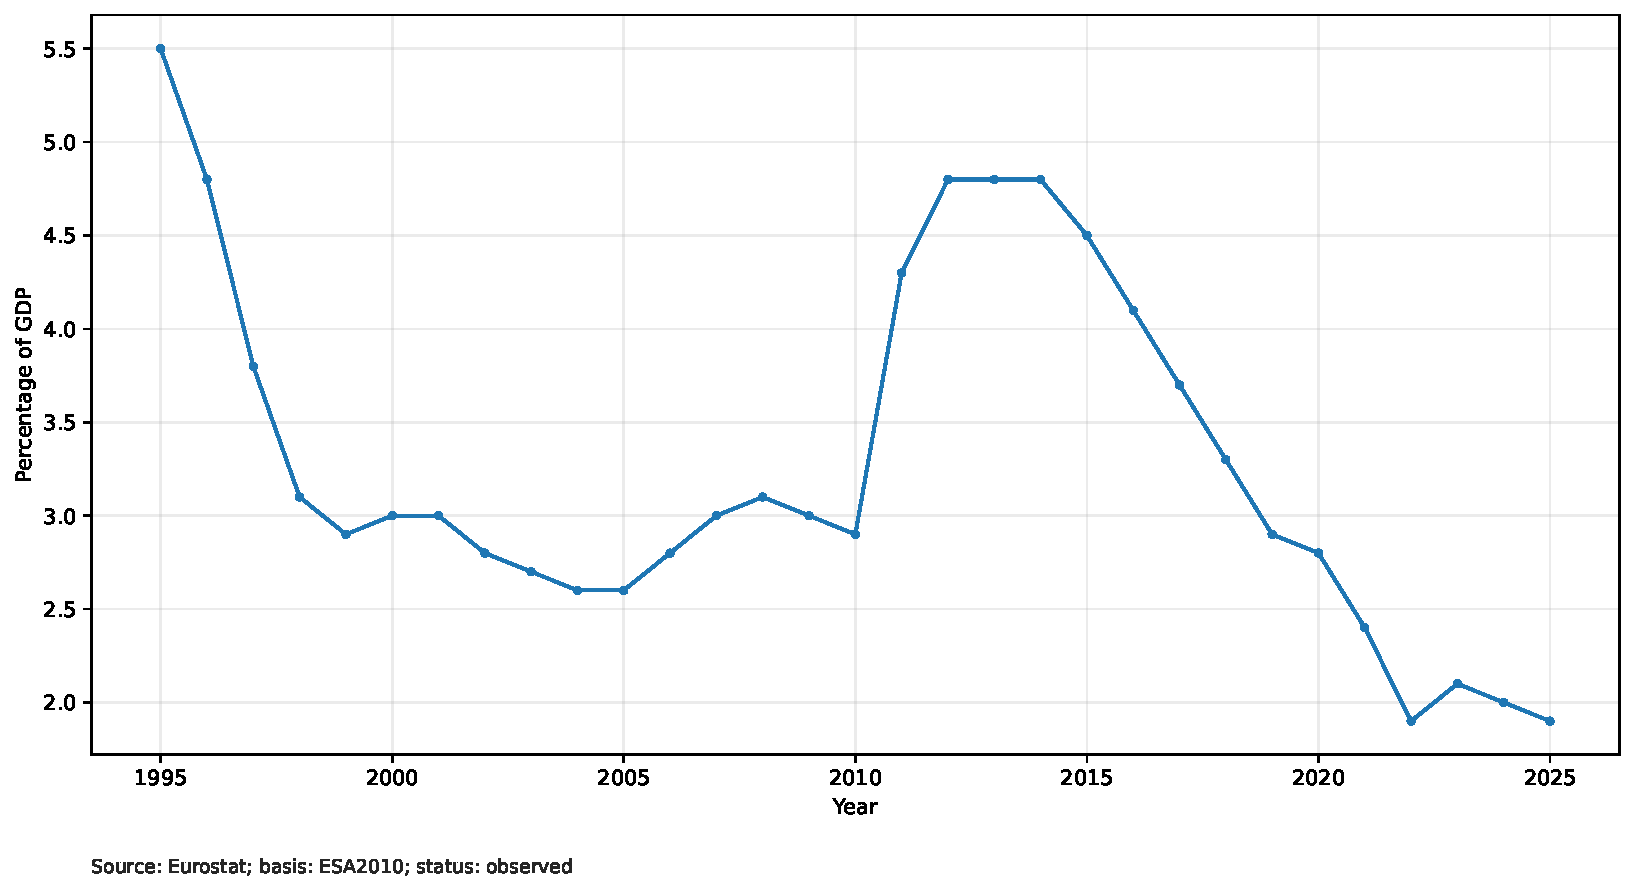
\includegraphics[width=0.9\textwidth]{../reports/figures/01_interest_pct_gdp.png}
\caption{Interest expenditure as a percentage of GDP.}
\label{fig:interest-gdp}
\end{figure}

\begin{figure}[H]
\centering
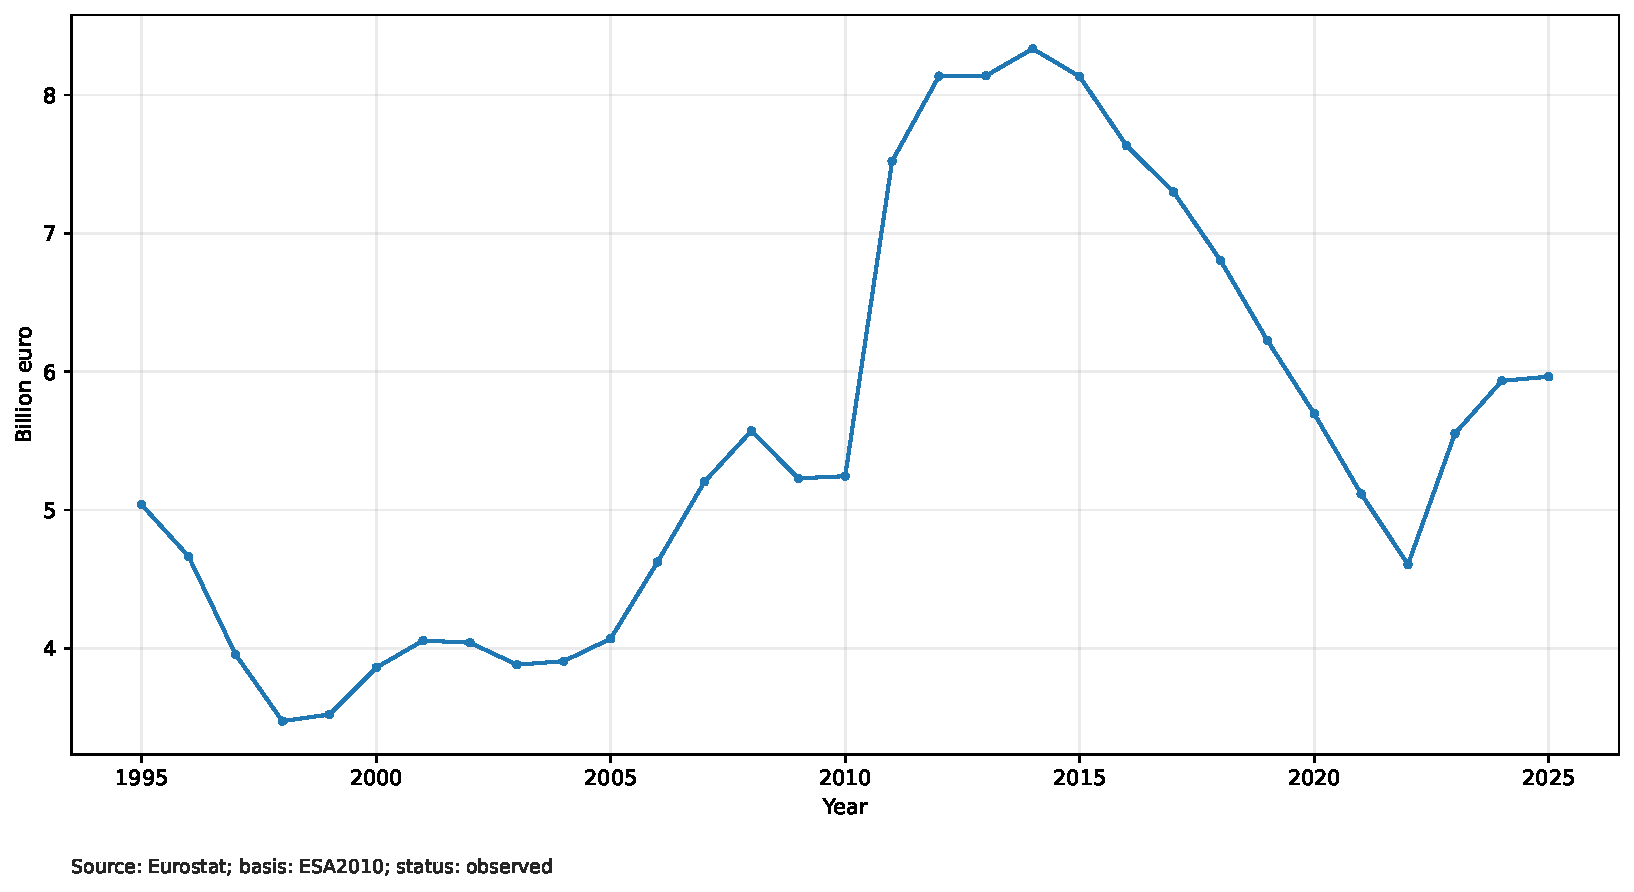
\includegraphics[width=0.9\textwidth]{../reports/figures/02_interest_billion_eur.png}
\caption{Interest expenditure in billion euros.}
\label{fig:interest-eur}
\end{figure}

\begin{figure}[H]
\centering
\includegraphics[width=0.9\textwidth]{../reports/figures/03_debt_and_implicit_rate.png}
\caption{Debt ratio and implicit interest rate.}
\label{fig:debt-rate}
\end{figure}

\begin{figure}[H]
\centering
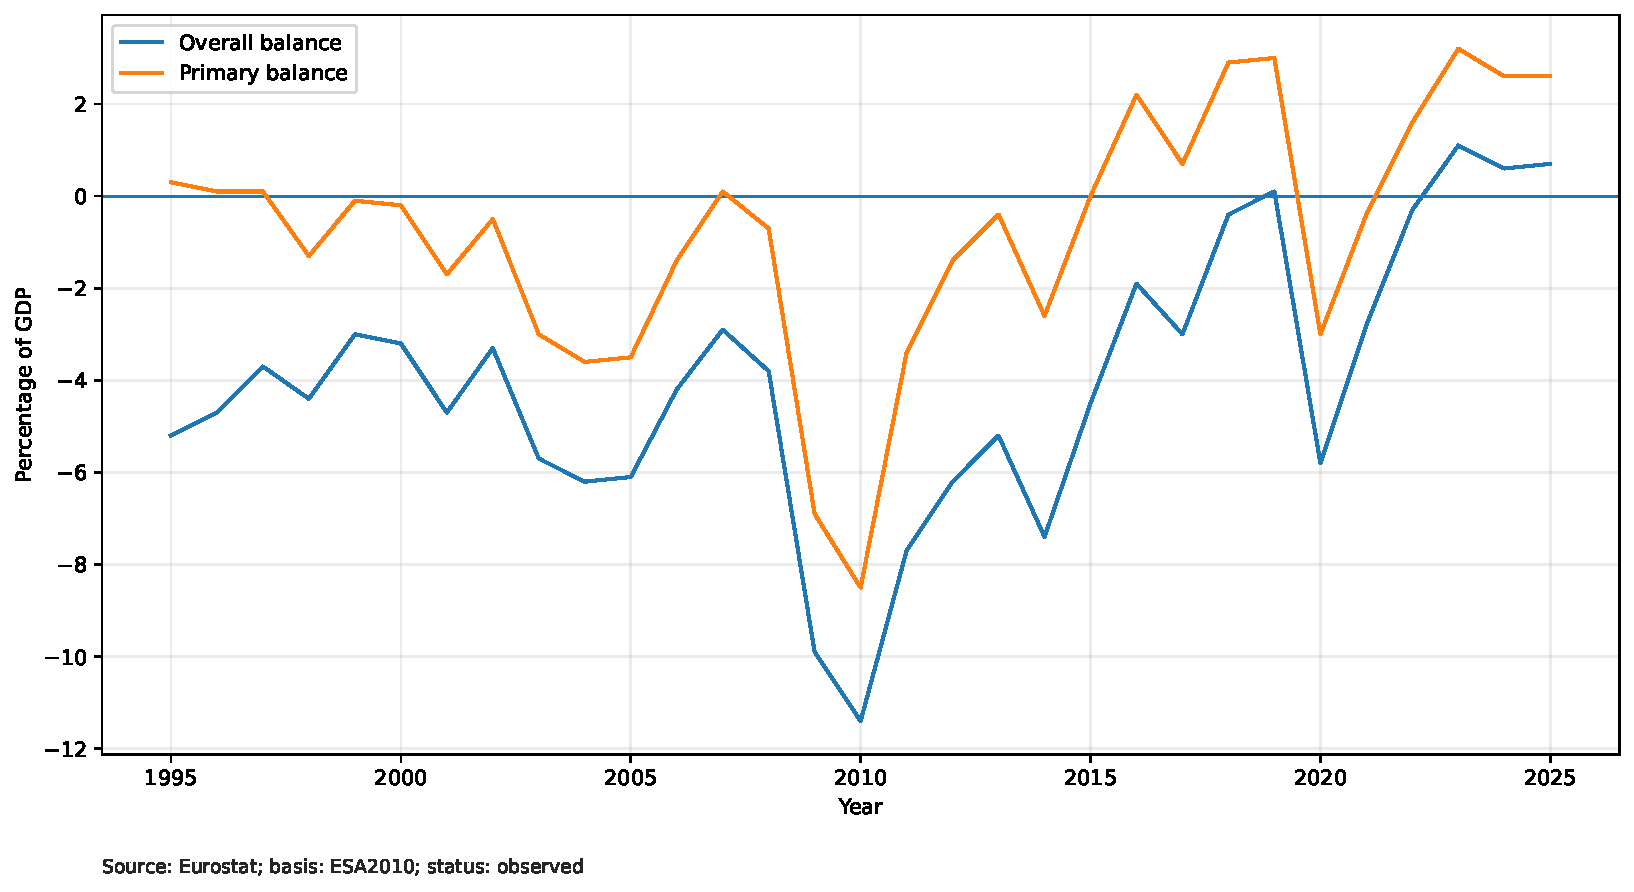
\includegraphics[width=0.9\textwidth]{../reports/figures/04_overall_and_primary_balance.png}
\caption{Overall and primary balances.}
\label{fig:balances}
\end{figure}

\begin{figure}[H]
\centering
\includegraphics[width=0.9\textwidth]{../reports/figures/05_market_yield_vs_implicit_rate.png}
\caption{Benchmark market yield versus implicit interest rate.}
\label{fig:yield-pass-through}
\end{figure}

\begin{figure}[H]
\centering
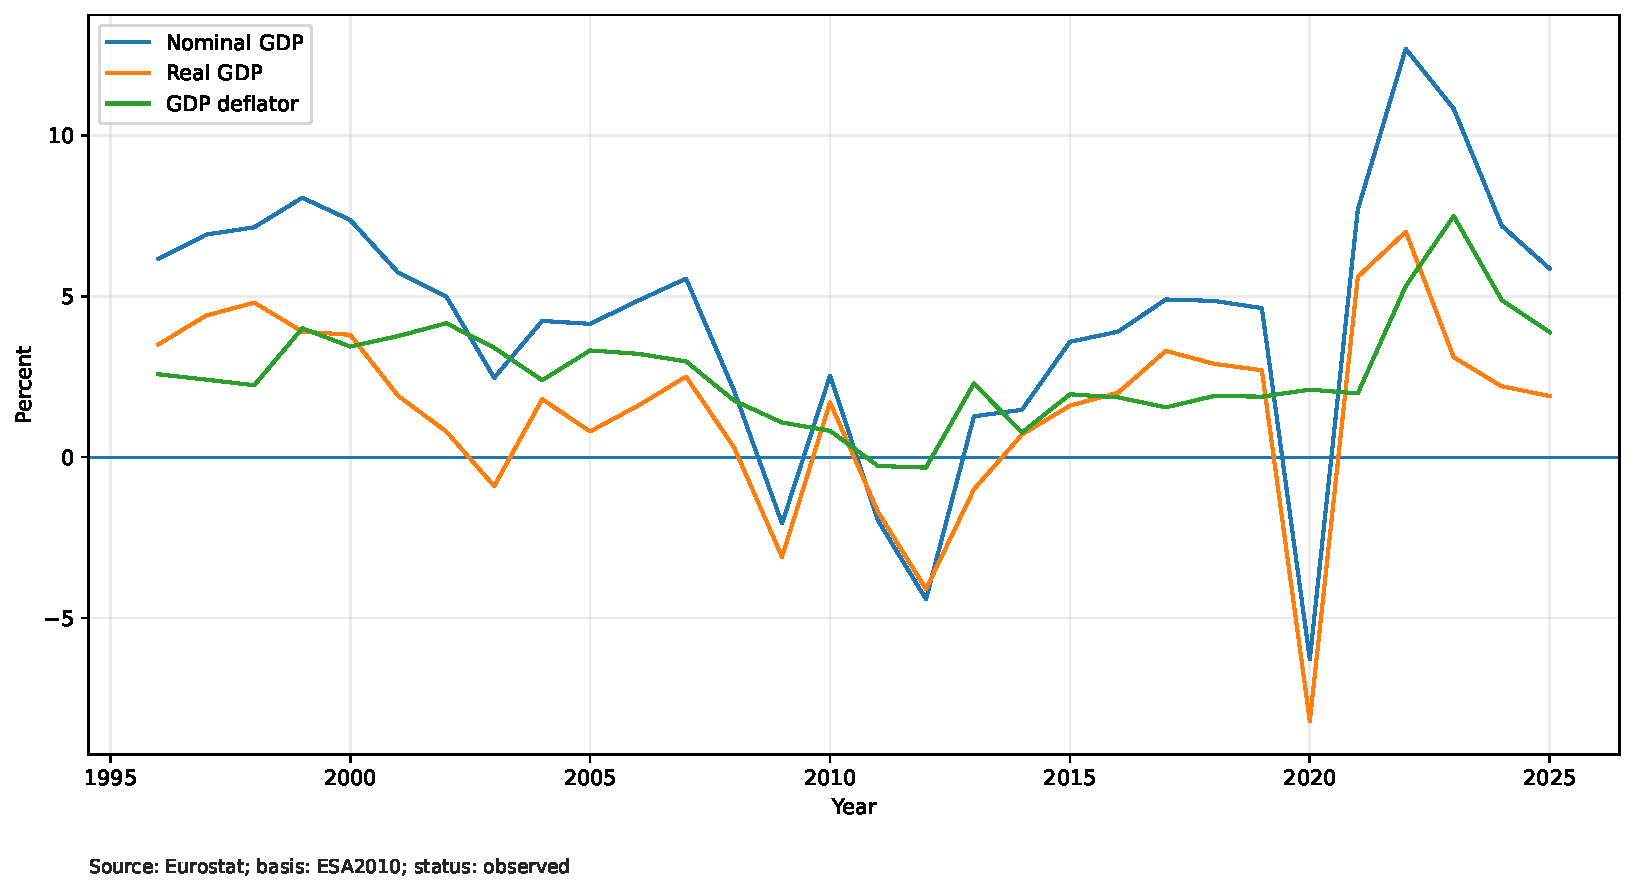
\includegraphics[width=0.9\textwidth]{../reports/figures/06_growth_decomposition.png}
\caption{Nominal growth, real growth, and GDP-deflator growth.}
\label{fig:growth}
\end{figure}

\begin{figure}[H]
\centering
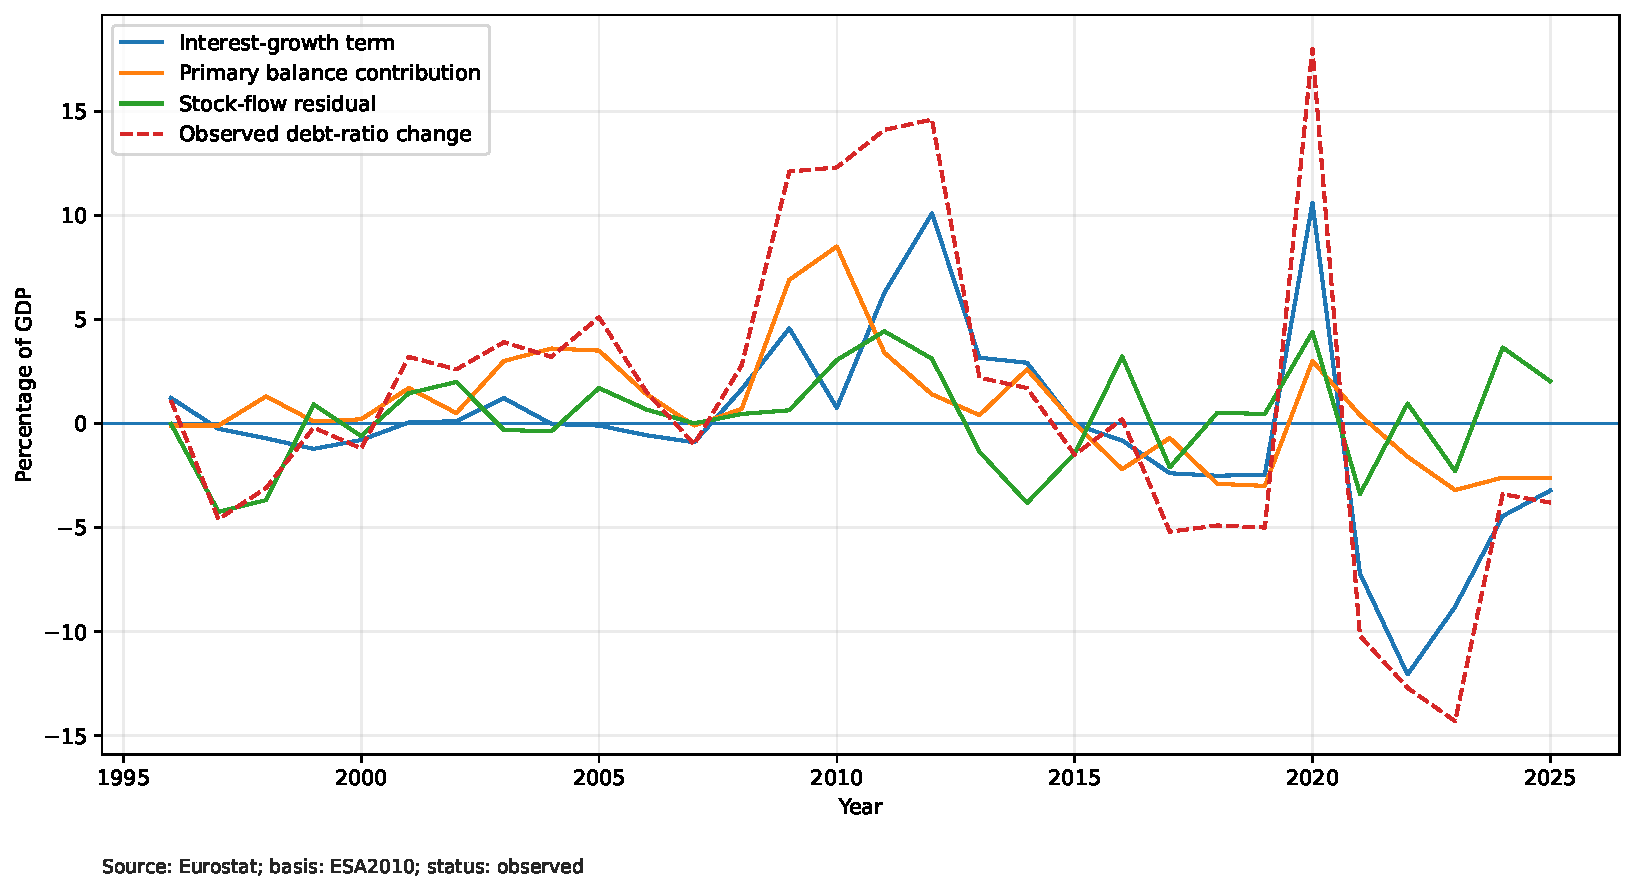
\includegraphics[width=0.9\textwidth]{../reports/figures/07_debt_dynamics.png}
\caption{Debt-dynamics decomposition.}
\label{fig:debt-dynamics}
\end{figure}

\section{European Comparison}

The comparator panel uses the same Eurostat concepts, units, and sector filters
as the Portugal series. Aggregate geographies such as the euro area are retained
for context but excluded from country ranks. In the 2025 panel Portugal ranked
fourth of seven non-aggregate comparator countries by interest expenditure as a
percentage of GDP.

\begin{table}[H]
\centering
\caption{Comparator panel, latest observed year}
\label{tab:panel}
\begin{tabular}{llrrrr}
\toprule
Rank & Geography & Interest/GDP & Debt/GDP & Implicit rate & Code \\
 & & (\%) & (\%) & (\%) & \\
\midrule
1 & Italy & 3.9 & 137.1 & 2.87 & IT \\
2 & Greece & 3.2 & 146.1 & 2.15 & EL \\
3 & Spain & 2.4 & 100.7 & 2.43 & ES \\
4 & Portugal & 1.9 & 89.7 & 2.18 & PT \\
5 & Germany & 1.1 & 63.5 & 1.79 & DE \\
6 & Netherlands & 0.7 & 44.4 & 1.67 & NL \\
7 & Ireland & 0.5 & 32.9 & 1.40 & IE \\
\bottomrule
\end{tabular}
\end{table}

\begin{figure}[H]
\centering
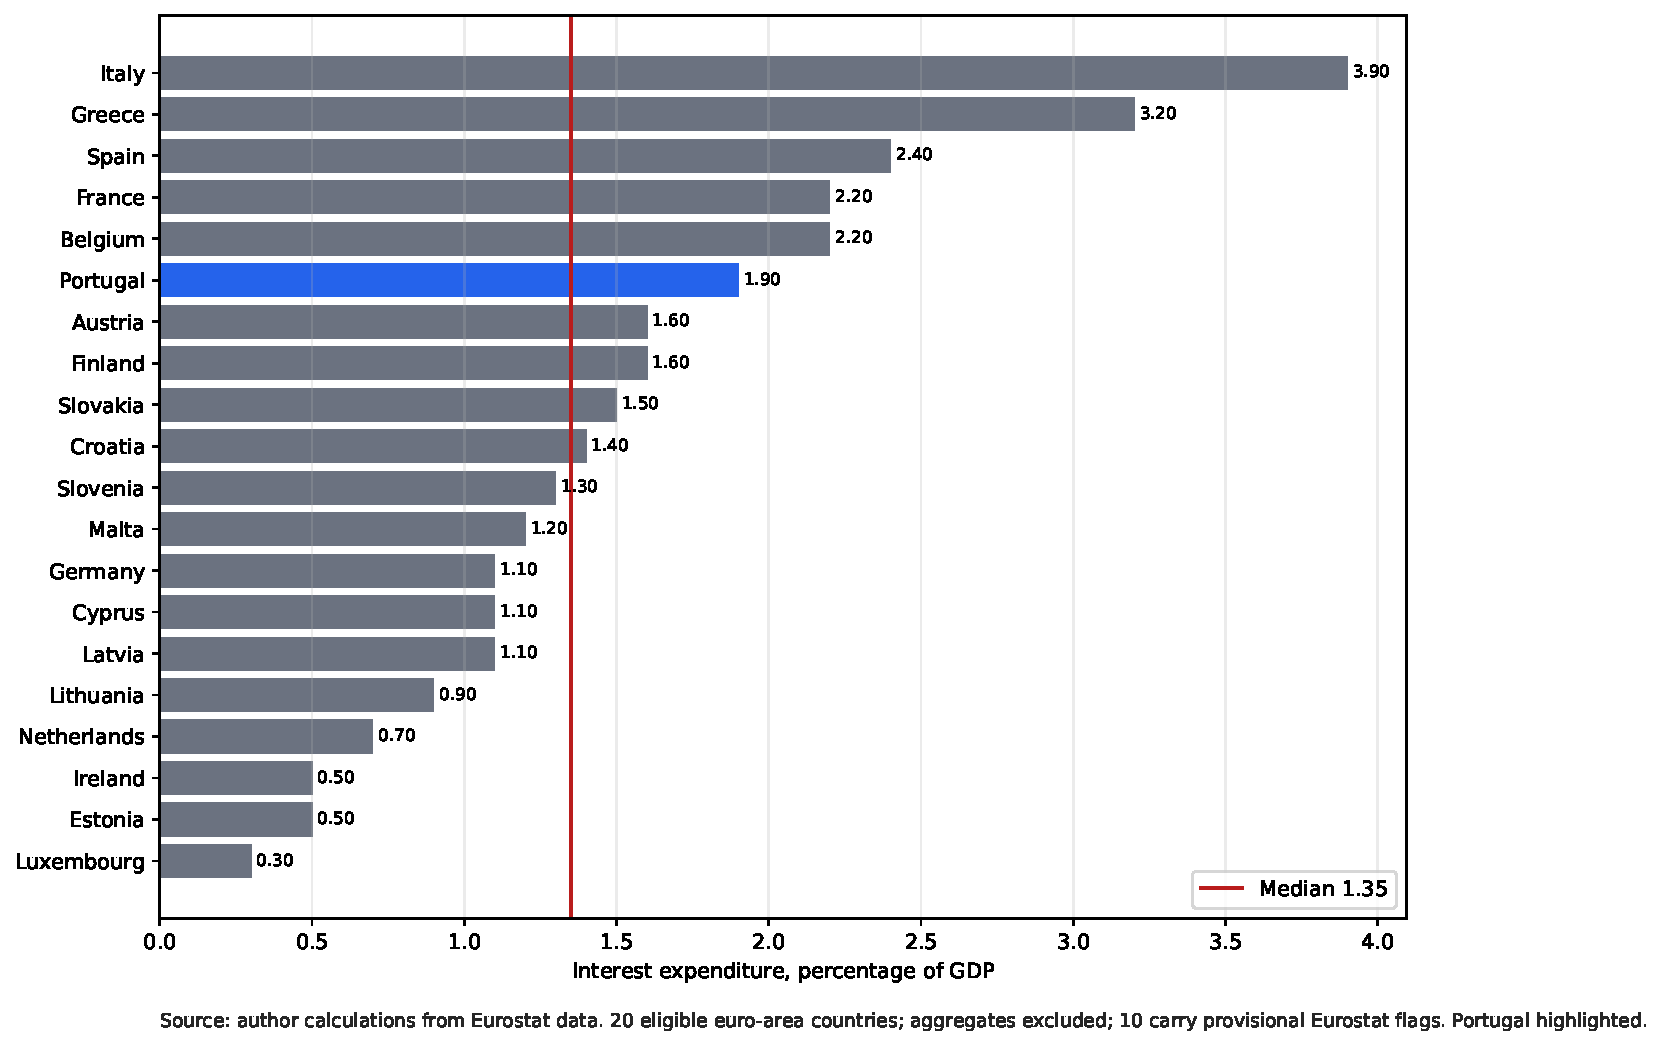
\includegraphics[width=0.9\textwidth]{../reports/figures/08_european_comparison.png}
\caption{European comparison of interest expenditure as a percentage of GDP.}
\label{fig:europe}
\end{figure}

\section{Rate-Shock Simulations}

The static simulation applies a rate shock to the entire debt stock:
\begin{equation}
  \Delta b = d \Delta r.
\end{equation}
At the 2025 debt ratio of 89.70 percent of GDP, a full pass-through of 100 basis
points implies an arithmetic increase in the interest burden of approximately
0.90 percentage points of GDP. The 50 and 200 basis-point shocks imply
approximately 0.45 and 1.79 percentage points, respectively. These are long-run
arithmetic effects, not one-year forecasts.

\begin{table}[H]
\centering
\caption{Static full-pass-through sensitivities}
\label{tab:shock}
\begin{tabular}{rrrr}
\toprule
Debt/GDP & Shock & Shock rate & Additional interest/GDP \\
(\%) & (bps) & decimal & (pp) \\
\midrule
89.70 & 50 & 0.005 & 0.449 \\
89.70 & 100 & 0.010 & 0.897 \\
89.70 & 200 & 0.020 & 1.794 \\
\bottomrule
\end{tabular}
\end{table}

\begin{figure}[H]
\centering
\includegraphics[width=0.9\textwidth]{../reports/figures/09_refinancing_shock_paths.png}
\caption{Gradual refinancing shock paths.}
\label{fig:refinancing}
\end{figure}

\section{Interpretation}

The central empirical finding is that Portugal's interest burden has fallen
substantially from the mid-1990s and from the sovereign-debt-crisis peak. This
decline should not be read as a simple decline in the euro amount of interest
paid. Instead, it reflects several interacting mechanisms:
\begin{enumerate}
  \item lower effective interest rates on the outstanding stock after the
        sovereign-debt crisis and the ECB intervention period;
  \item strong nominal GDP growth in the post-pandemic and inflation period;
  \item a declining debt ratio after the 2020 pandemic peak;
  \item positive primary balances in recent years;
  \item gradual rather than immediate pass-through from market yields to the
        average cost of the debt stock.
\end{enumerate}

The European comparison places Portugal in an intermediate position. Its 2025
interest burden is below Italy, Greece, and Spain, but above Germany, the
Netherlands, and Ireland. This ranking is consistent with Portugal's still-high
but declining debt ratio and an implicit rate that remains moderate relative to
the countries with the largest burdens.

\section{Limitations}

Several limitations should govern interpretation. First, pre-1995 observations
are linked AMECO observations and do not have the same accounting status as the
ESA 2010 Eurostat main series. Second, interest payable under ESA is not
identical to central-government cash interest or to newly issued bond yields.
Third, rate-shock simulations are deterministic arithmetic exercises; they do
not model feedback from fiscal policy, maturity management, risk premia,
inflation, or economic growth. Fourth, the stock-flow adjustment is a residual
and should be interpreted as a reconciliation term, not a structural causal
estimate. Finally, cross-country comparisons are harmonised by Eurostat
definitions but do not adjust for all country-level debt-management differences.

\section{Conclusion}

Portugal's public-debt interest burden has moved from a high-burden environment
in the mid-1990s and sovereign-debt-crisis period to a much lower burden in the
current dataset. The 2025 interest bill remains economically material at EUR
5.96 billion, but the GDP burden is 1.90 percent, supported by a lower debt
ratio and nominal growth. The main fiscal risk is not that market-rate increases
immediately reprice the entire stock, but that sustained higher rates gradually
raise the effective cost as debt is refinanced. The reproducible pipeline and
validation checks in this repository make that distinction explicit and provide
a basis for future updates as Eurostat and AMECO revise source data.

\appendix

\section{Validation Appendix}

The latest validation result passed all error-severity checks. One warning was
recorded: official and calculated debt ratios differed by more than 0.15
percentage points in 1997 and 1998. This is retained as an audit item.

\section{Reproducibility Appendix}

The report was prepared from the repository-local processed outputs generated by:
\begin{verbatim}
python -m pt_debt_interest.cli all --config config/default.yaml
\end{verbatim}

The local quality checks were:
\begin{verbatim}
pytest
ruff check .
mypy src
\end{verbatim}

\section{Source Notes}

Eurostat datasets used by the pipeline include \texttt{gov\_10a\_main},
\texttt{gov\_10dd\_edpt1}, \texttt{nama\_10\_gdp}, and
\texttt{irt\_lt\_mcby\_a}. AMECO is used only for the linked historical
extension and is preserved with explicit source and accounting-basis metadata.

\end{document}
